\documentclass[12pt]{extarticle}
\usepackage[dvipsnames]{xcolor}
\usepackage{xeCJK}
\usepackage{hyperref}
\usepackage{graphicx}
\usepackage{amsmath}
\usepackage{tikz}


\hypersetup{
    colorlinks=true,        % Use colored text instead of boxes
}

\title{RL HW1 Report}
\author{Yu-Xiang, Luo}

\begin{document}

\maketitle
\section*{Q1}
What methods have you tried for async DP? Compare their performance.\\
\\
Unfortunately, I did not come out a way to implement prioritized sweeping and real-time DP. I can only perform the in-place DP.
\begin{itemize}
	\item in-place DP: \textcolor{ForestGreen}{\textbf{Iteration steps: 968}}, the value iteration sync DP is \textcolor{ForestGreen}{\textbf{1056}} steps
	\item Prioritized sweeping: \textcolor{gray}{No implementation}
	\item Real-time DP: \textcolor{gray}{No implementation}
\end{itemize}
\newpage
The reason why in-place DP is effective:
Let's consider a simple scenario: a $n \times 1$ grid world, with $\text{S}_{n-1}$ be goal state.

\[
	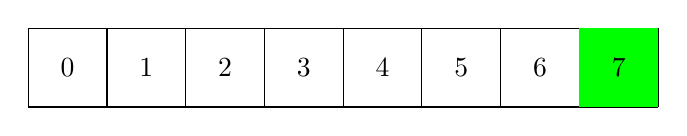
\begin{tikzpicture}
		% Draw horizontal lines
		\foreach \y in {0,1}
		\draw (0,\y) -- (8,\y);

		% Draw vertical lines
		\foreach \x in {0,1,2,3,4,5,6,7,8}
		\draw (\x,0) -- (\x,1);
		\node at (0.5, 0.5) {0};
		\node at (1.5, 0.5) {1};
		\node at (2.5, 0.5) {2};
		\node at (3.5, 0.5) {3};
		\node at (4.5, 0.5) {4};
		\node at (5.5, 0.5) {5};
		\node at (6.5, 0.5) {6};
		\fill[green] (7,0) rectangle (8,1);
		\node at (7.5, 0.5) {7};
	\end{tikzpicture}
\]
\[
	\texttt{step\_reward = -1, goal\_reward = 10}
\]
\[
	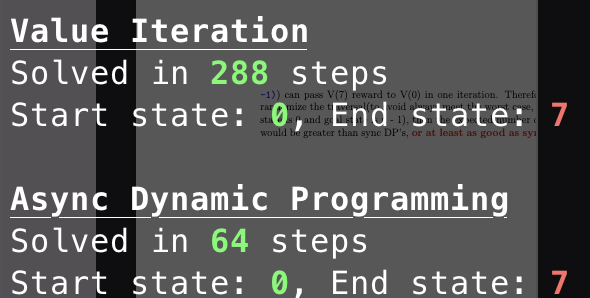
\includegraphics[width=0.8\textwidth]{./img/experiment_log.png}
\]
\[
	\textbf{\textcolor{red}{\text{The async DP use }\texttt{[i for i in range(7, -1, -1)]}\text{ as Iteration order}}}
\]

This is a simple case, but I think is enough to explain my thought. Initailly, $\forall v \in V, v = 0$, which means in the first iteration, only V(7) is changed since \texttt{\textcolor{blue}{step(7, action).reward = 1}}. While, at the second iteration, sync DP will only change the value of V(6) since only V(7) change. Then, V(5) and V(6), during next iterations. In other words, The reward of V(7) needs at least 7 iteratios to pass through V(0), yet in in-place DP, the best traverse order(\texttt{\textcolor{blue}{for i in range(7, -1, -1)}}) can pass V(7) reward to V(0) in one iteration. Therefore, if we randomize the traversal(to avoid always meet the worst case, like start state is 0 and goal state is n - 1), then the expected number of update would be greater than sync DP's, \textbf{\textcolor{red}{or at least as good as sync DP's}}.(Sometimes it doesn't improve because the reward isn't good enough for the agent. Like the default reward for our HW1, step\_reward = -1, goal\_reward = 1 is not enough)

\[
	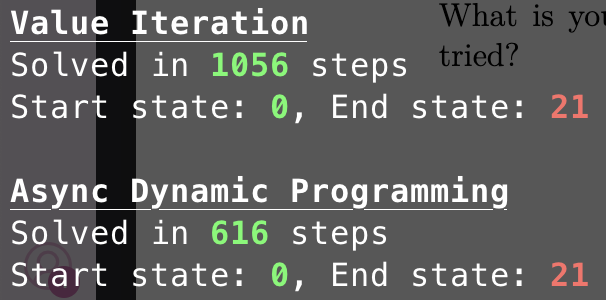
\includegraphics[width=\textwidth]{./img/exp2.png}
\]
\[
	\text{Randomize the order of traversal in every iteration, \texttt{goal\_reward = 100}}
\]
\[
	\text{I do try this method on the maze TA offer, and the result is as above.}
\]

\newpage
\section*{Q2}
What is your final method? How is it better than other methods you've tried?\\
\\
Since we're allowed to store all step we've travelled. That is, we can store all \texttt{grid\_world.step(state, action)}. Then, the worst iteration steps would be \textcolor{red}{4 * \textit{state\_space}}.

\[
	\fbox{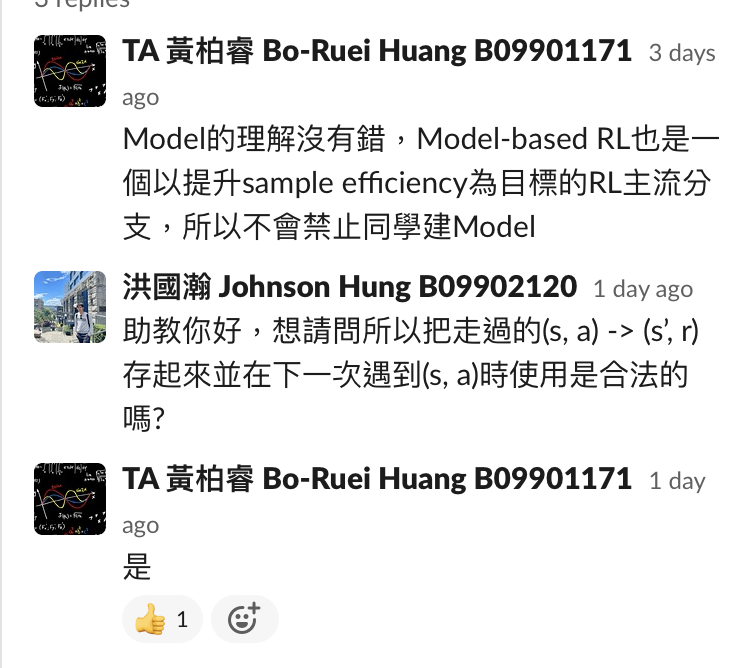
\includegraphics[width=\textwidth]{./img/discussion.png}}
\]

By little improvement, step on goal state and trap state can be reduced to 1.

\end{document}

